\documentclass[tikz,border=10pt]{standalone}
\usepackage{amsmath}
\usetikzlibrary{shapes.geometric, arrows.meta, shadings}

\begin{document}
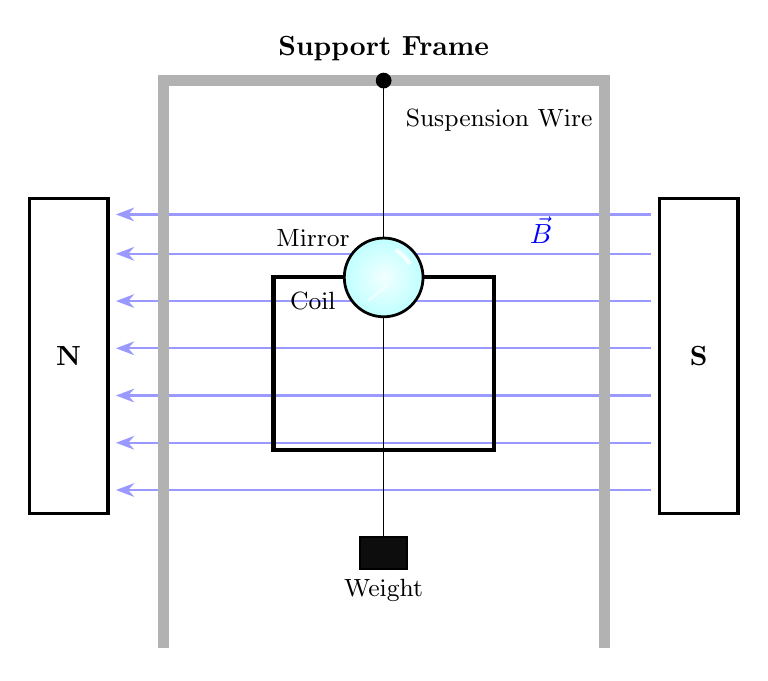
\begin{tikzpicture}[>=Stealth, thick]

    \draw [line width=1.2pt] (-4.5, 0.5) rectangle (-3.5, 4.5);
    \node at (-4.0, 2.5) {\textbf{N}};
    
    \draw [line width=1.2pt] (4.5, 0.5) rectangle (3.5, 4.5);
    \node at (4.0, 2.5) {\textbf{S}};

    \foreach \y in {0.8, 1.4, ..., 3.8, 4.3} {
        \draw [->, blue!40, line width=0.8pt] (3.4, \y) -- (-3.4, \y);
    }
    \node [blue] at (2, 4.1) {$\vec{B}$};

    % --- 3. Extra Thick Support Frame (支架 4pt) ---
    \draw [line width=4pt, color=gray!60] (-2.8,-1.2) -- (-2.8,6) -- (2.8,6) -- (2.8,-1.2);
    \node at (0,6.4) {\textbf{Support Frame}};

    % --- 4. Suspension Wire (贯穿细线) ---
    % 延长至横向配重的顶部 (y=0.2)
    \draw [line width=0.6pt] (0,6) -- (0,0.2);
    \fill [black] (0,6) circle (0.1);
    \node [right] at (0.15,5.5) {\small Suspension Wire};

    % --- 5. Enlarged Rectangular Coil Frame (Aspect Ratio 55:43) ---
    % 宽度 2.8, 高度 2.19 (y: 3.5 down to 1.31)
    \draw [line width=1.5pt] (-1.4, 1.31) rectangle (1.4, 3.5);
    \node at (-0.9, 3.2) {\small Coil};

    % --- 6. Optical Mirror (Glass/Glint Effects) ---
    \begin{scope}
        \clip (0,3.5) circle (0.5);
        \shade [inner color=cyan!5, outer color=cyan!25] (0,3.5) circle (0.5);
    \end{scope}
    \draw [line width=1pt] (0,3.5) circle (0.5);
    
    % 高光效果
    \draw [white, line width=1.5pt, opacity=0.8] (0.15, 3.85) arc (60:30:0.5);
    \draw [white, line width=0.8pt, opacity=0.6] (-0.2, 3.2) -- (0.05, 3.4);
    \node [left] at (-0.3, 4) {\small Mirror};

    % --- 7. Rotated Counterweight (横向长方形配重) ---
    % 旋转90度后，宽度设为 0.6，高度设为 0.4
    % 顶部连接在 y=0.2，底部到 y=-0.2
    \draw [fill=black!95] (-0.3, -0.2) rectangle (0.3, 0.2);
    \node [below] at (0, -0.2) {\small Weight};

\end{tikzpicture}
\end{document}